
%% bare_jrnl_comsoc.tex
%% V1.4b
%% 2015/08/26
%% by Michael Shell
%% see http://www.michaelshell.org/
%% for current contact information.
%%
%% This is a skeleton file demonstrating the use of IEEEtran.cls
%% (requires IEEEtran.cls version 1.8b or later) with an IEEE
%% Communications Society journal paper.
%%
%% Support sites:
%% http://www.michaelshell.org/tex/ieeetran/
%% http://www.ctan.org/pkg/ieeetran
%% and
%% http://www.ieee.org/

%%*************************************************************************
%% Legal Notice:
%% This code is offered as-is without any warranty either expressed or
%% implied; without even the implied warranty of MERCHANTABILITY or
%% FITNESS FOR A PARTICULAR PURPOSE! 
%% User assumes all risk.
%% In no event shall the IEEE or any contributor to this code be liable for
%% any damages or losses, including, but not limited to, incidental,
%% consequential, or any other damages, resulting from the use or misuse
%% of any information contained here.
%%
%% All comments are the opinions of their respective authors and are not
%% necessarily endorsed by the IEEE.
%%
%% This work is distributed under the LaTeX Project Public License (LPPL)
%% ( http://www.latex-project.org/ ) version 1.3, and may be freely used,
%% distributed and modified. A copy of the LPPL, version 1.3, is included
%% in the base LaTeX documentation of all distributions of LaTeX released
%% 2003/12/01 or later.
%% Retain all contribution notices and credits.
%% ** Modified files should be clearly indicated as such, including  **
%% ** renaming them and changing author support contact information. **
%%*************************************************************************


% *** Authors should verify (and, if needed, correct) their LaTeX system  ***
% *** with the testflow diagnostic prior to trusting their LaTeX platform ***
% *** with production work. The IEEE's font choices and paper sizes can   ***
% *** trigger bugs that do not appear when using other class files.       ***                          ***
% The testflow support page is at:
% http://www.michaelshell.org/tex/testflow/



\documentclass[journal,comsoc]{IEEEtran}
%
% If IEEEtran.cls has not been installed into the LaTeX system files,
% manually specify the path to it like:
% \documentclass[journal,comsoc]{../sty/IEEEtran}


\usepackage[T1]{fontenc}% optional T1 font encoding


% *** MISC UTILITY PACKAGES ***
%
%\usepackage{ifpdf}
% Heiko Oberdiek's ifpdf.sty is very useful if you need conditional
% compilation based on whether the output is pdf or dvi.
% usage:
% \ifpdf
%   % pdf code
% \else
%   % dvi code
% \fi
% The latest version of ifpdf.sty can be obtained from:
% http://www.ctan.org/pkg/ifpdf
% Also, note that IEEEtran.cls V1.7 and later provides a builtin
% \ifCLASSINFOpdf conditional that works the same way.
% When switching from latex to pdflatex and vice-versa, the compiler may
% have to be run twice to clear warning/error messages.

% *** GRAPHIC PAKAGES *** 

\usepackage{graphicx}
\graphicspath{ {img/} }




% *** CITATION PACKAGES ***
%
%\usepackage{cite}
% cite.sty was written by Donald Arseneau
% V1.6 and later of IEEEtran pre-defines the format of the cite.sty package
% \cite{} output to follow that of the IEEE. Loading the cite package will
% result in citation numbers being automatically sorted and properly
% "compressed/ranged". e.g., [1], [9], [2], [7], [5], [6] without using
% cite.sty will become [1], [2], [5]--[7], [9] using cite.sty. cite.sty's
% \cite will automatically add leading space, if needed. Use cite.sty's
% noadjust option (cite.sty V3.8 and later) if you want to turn this off
% such as if a citation ever needs to be enclosed in parenthesis.
% cite.sty is already installed on most LaTeX systems. Be sure and use
% version 5.0 (2009-03-20) and later if using hyperref.sty.
% The latest version can be obtained at:
% http://www.ctan.org/pkg/cite
% The documentation is contained in the cite.sty file itself.






% *** GRAPHICS RELATED PACKAGES ***
%
\ifCLASSINFOpdf
  % \usepackage[pdftex]{graphicx}
  % declare the path(s) where your graphic files are
  % \graphicspath{{../pdf/}{../jpeg/}}
  % and their extensions so you won't have to specify these with
  % every instance of \includegraphics
  % \DeclareGraphicsExtensions{.pdf,.jpeg,.png}
\else
  % or other class option (dvipsone, dvipdf, if not using dvips). graphicx
  % will default to the driver specified in the system graphics.cfg if no
  % driver is specified.
  % \usepackage[dvips]{graphicx}
  % declare the path(s) where your graphic files are
  % \graphicspath{{../eps/}}
  % and their extensions so you won't have to specify these with
  % every instance of \includegraphics
  % \DeclareGraphicsExtensions{.eps}
\fi
% graphicx was written by David Carlisle and Sebastian Rahtz. It is
% required if you want graphics, photos, etc. graphicx.sty is already
% installed on most LaTeX systems. The latest version and documentation
% can be obtained at: 
% http://www.ctan.org/pkg/graphicx
% Another good source of documentation is "Using Imported Graphics in
% LaTeX2e" by Keith Reckdahl which can be found at:
% http://www.ctan.org/pkg/epslatex
%
% latex, and pdflatex in dvi mode, support graphics in encapsulated
% postscript (.eps) format. pdflatex in pdf mode supports graphics
% in .pdf, .jpeg, .png and .mps (metapost) formats. Users should ensure
% that all non-photo figures use a vector format (.eps, .pdf, .mps) and
% not a bitmapped formats (.jpeg, .png). The IEEE frowns on bitmapped formats
% which can result in "jaggedy"/blurry rendering of lines and letters as
% well as large increases in file sizes.
%
% You can find documentation about the pdfTeX application at:
% http://www.tug.org/applications/pdftex





% *** MATH PACKAGES ***
%
\usepackage{amsmath}
% A popular package from the American Mathematical Society that provides
% many useful and powerful commands for dealing with mathematics.
% Do NOT use the amsbsy package under comsoc mode as that feature is
% already built into the Times Math font (newtxmath, mathtime, etc.).
% 
% Also, note that the amsmath package sets \interdisplaylinepenalty to 10000
% thus preventing page breaks from occurring within multiline equations. Use:
\interdisplaylinepenalty=2500
% after loading amsmath to restore such page breaks as IEEEtran.cls normally
% does. amsmath.sty is already installed on most LaTeX systems. The latest
% version and documentation can be obtained at:
% http://www.ctan.org/pkg/amsmath


% Select a Times math font under comsoc mode or else one will automatically
% be selected for you at the document start. This is required as Communications
% Society journals use a Times, not Computer Modern, math font.
\usepackage[cmintegrals]{newtxmath}
% The freely available newtxmath package was written by Michael Sharpe and
% provides a feature rich Times math font. The cmintegrals option, which is
% the default under IEEEtran, is needed to get the correct style integral
% symbols used in Communications Society journals. Version 1.451, July 28,
% 2015 or later is recommended. Also, do *not* load the newtxtext.sty package
% as doing so would alter the main text font.
% http://www.ctan.org/pkg/newtx
%
% Alternatively, you can use the MathTime commercial fonts if you have them
% installed on your system:
%\usepackage{mtpro2}
%\usepackage{mt11p}
%\usepackage{mathtime}


%\usepackage{bm}
% The bm.sty package was written by David Carlisle and Frank Mittelbach.
% This package provides a \bm{} to produce bold math symbols.
% http://www.ctan.org/pkg/bm





% *** SPECIALIZED LIST PACKAGES ***
%
%\usepackage{algorithmic}
% algorithmic.sty was written by Peter Williams and Rogerio Brito.
% This package provides an algorithmic environment fo describing algorithms.
% You can use the algorithmic environment in-text or within a figure
% environment to provide for a floating algorithm. Do NOT use the algorithm
% floating environment provided by algorithm.sty (by the same authors) or
% algorithm2e.sty (by Christophe Fiorio) as the IEEE does not use dedicated
% algorithm float types and packages that provide these will not provide
% correct IEEE style captions. The latest version and documentation of
% algorithmic.sty can be obtained at:
% http://www.ctan.org/pkg/algorithms
% Also of interest may be the (relatively newer and more customizable)
% algorithmicx.sty package by Szasz Janos:
% http://www.ctan.org/pkg/algorithmicx




% *** ALIGNMENT PACKAGES ***
%
%\usepackage{array}
% Frank Mittelbach's and David Carlisle's array.sty patches and improves
% the standard LaTeX2e array and tabular environments to provide better
% appearance and additional user controls. As the default LaTeX2e table
% generation code is lacking to the point of almost being broken with
% respect to the quality of the end results, all users are strongly
% advised to use an enhanced (at the very least that provided by array.sty)
% set of table tools. array.sty is already installed on most systems. The
% latest version and documentation can be obtained at:
% http://www.ctan.org/pkg/array


% IEEEtran contains the IEEEeqnarray family of commands that can be used to
% generate multiline equations as well as matrices, tables, etc., of high
% quality.




% *** SUBFIGURE PACKAGES ***
%\ifCLASSOPTIONcompsoc
%  \usepackage[caption=false,font=normalsize,labelfont=sf,textfont=sf]{subfig}
%\else
%  \usepackage[caption=false,font=footnotesize]{subfig}
%\fi
% subfig.sty, written by Steven Douglas Cochran, is the modern replacement
% for subfigure.sty, the latter of which is no longer maintained and is
% incompatible with some LaTeX packages including fixltx2e. However,
% subfig.sty requires and automatically loads Axel Sommerfeldt's caption.sty
% which will override IEEEtran.cls' handling of captions and this will result
% in non-IEEE style figure/table captions. To prevent this problem, be sure
% and invoke subfig.sty's "caption=false" package option (available since
% subfig.sty version 1.3, 2005/06/28) as this is will preserve IEEEtran.cls
% handling of captions.
% Note that the Computer Society format requires a larger sans serif font
% than the serif footnote size font used in traditional IEEE formatting
% and thus the need to invoke different subfig.sty package options depending
% on whether compsoc mode has been enabled.
%
% The latest version and documentation of subfig.sty can be obtained at:
% http://www.ctan.org/pkg/subfig




% *** FLOAT PACKAGES ***
%
%\usepackage{fixltx2e}
% fixltx2e, the successor to the earlier fix2col.sty, was written by
% Frank Mittelbach and David Carlisle. This package corrects a few problems
% in the LaTeX2e kernel, the most notable of which is that in current
% LaTeX2e releases, the ordering of single and double column floats is not
% guaranteed to be preserved. Thus, an unpatched LaTeX2e can allow a
% single column figure to be placed prior to an earlier double column
% figure.
% Be aware that LaTeX2e kernels dated 2015 and later have fixltx2e.sty's
% corrections already built into the system in which case a warning will
% be issued if an attempt is made to load fixltx2e.sty as it is no longer
% needed.
% The latest version and documentation can be found at:
% http://www.ctan.org/pkg/fixltx2e


%\usepackage{stfloats}
% stfloats.sty was written by Sigitas Tolusis. This package gives LaTeX2e
% the ability to do double column floats at the bottom of the page as well
% as the top. (e.g., "\begin{figure*}[!b]" is not normally possible in
% LaTeX2e). It also provides a command:
%\fnbelowfloat
% to enable the placement of footnotes below bottom floats (the standard
% LaTeX2e kernel puts them above bottom floats). This is an invasive package
% which rewrites many portions of the LaTeX2e float routines. It may not work
% with other packages that modify the LaTeX2e float routines. The latest
% version and documentation can be obtained at:
% http://www.ctan.org/pkg/stfloats
% Do not use the stfloats baselinefloat ability as the IEEE does not allow
% \baselineskip to stretch. Authors submitting work to the IEEE should note
% that the IEEE rarely uses double column equations and that authors should try
% to avoid such use. Do not be tempted to use the cuted.sty or midfloat.sty
% packages (also by Sigitas Tolusis) as the IEEE does not format its papers in
% such ways.
% Do not attempt to use stfloats with fixltx2e as they are incompatible.
% Instead, use Morten Hogholm'a dblfloatfix which combines the features
% of both fixltx2e and stfloats:
%
% \usepackage{dblfloatfix}
% The latest version can be found at:
% http://www.ctan.org/pkg/dblfloatfix




%\ifCLASSOPTIONcaptionsoff
%  \usepackage[nomarkers]{endfloat}
% \let\MYoriglatexcaption\caption
% \renewcommand{\caption}[2][\relax]{\MYoriglatexcaption[#2]{#2}}
%\fi
% endfloat.sty was written by James Darrell McCauley, Jeff Goldberg and 
% Axel Sommerfeldt. This package may be useful when used in conjunction with 
% IEEEtran.cls'  captionsoff option. Some IEEE journals/societies require that
% submissions have lists of figures/tables at the end of the paper and that
% figures/tables without any captions are placed on a page by themselves at
% the end of the document. If needed, the draftcls IEEEtran class option or
% \CLASSINPUTbaselinestretch interface can be used to increase the line
% spacing as well. Be sure and use the nomarkers option of endfloat to
% prevent endfloat from "marking" where the figures would have been placed
% in the text. The two hack lines of code above are a slight modification of
% that suggested by in the endfloat docs (section 8.4.1) to ensure that
% the full captions always appear in the list of figures/tables - even if
% the user used the short optional argument of \caption[]{}.
% IEEE papers do not typically make use of \caption[]'s optional argument,
% so this should not be an issue. A similar trick can be used to disable
% captions of packages such as subfig.sty that lack options to turn off
% the subcaptions:
% For subfig.sty:
% \let\MYorigsubfloat\subfloat
% \renewcommand{\subfloat}[2][\relax]{\MYorigsubfloat[]{#2}}
% However, the above trick will not work if both optional arguments of
% the \subfloat command are used. Furthermore, there needs to be a
% description of each subfigure *somewhere* and endfloat does not add
% subfigure captions to its list of figures. Thus, the best approach is to
% avoid the use of subfigure captions (many IEEE journals avoid them anyway)
% and instead reference/explain all the subfigures within the main caption.
% The latest version of endfloat.sty and its documentation can obtained at:
% http://www.ctan.org/pkg/endfloat
%
% The IEEEtran \ifCLASSOPTIONcaptionsoff conditional can also be used
% later in the document, say, to conditionally put the References on a 
% page by themselves.




% *** PDF, URL AND HYPERLINK PACKAGES ***
%
\usepackage{url}
% url.sty was written by Donald Arseneau. It provides better support for
% handling and breaking URLs. url.sty is already installed on most LaTeX
% systems. The latest version and documentation can be obtained at:
% http://www.ctan.org/pkg/url
% Basically, \url{my_url_here}.




% *** Do not adjust lengths that control margins, column widths, etc. ***
% *** Do not use packages that alter fonts (such as pslatex).         ***
% There should be no need to do such things with IEEEtran.cls V1.6 and later.
% (Unless specifically asked to do so by the journal or conference you plan
% to submit to, of course. )


% correct bad hyphenation here
\hyphenation{op-tical net-works semi-conduc-tor}

\usepackage{hyperref}

\begin{document}
%
% paper title
% Titles are generally capitalized except for words such as a, an, and, as,
% at, but, by, for, in, nor, of, on, or, the, to and up, which are usually
% not capitalized unless they are the first or last word of the title.
% Linebreaks \\ can be used within to get better formatting as desired.
% Do not put math or special symbols in the title.
\title{Sweetie: a One to One app for couples}
%
%
% author names and IEEE memberships
% note positions of commas and nonbreaking spaces ( ~ ) LaTeX will not break
% a structure at a ~ so this keeps an author's name from being broken across
% two lines.
% use \thanks{} to gain access to the first footnote area
% a separate \thanks must be used for each paragraph as LaTeX2e's \thanks
% was not built to handle multiple paragraphs
%

\author{Federico~Ghirardelli,~\IEEEmembership{Computer Science Master Degree,~federico.ghirardelli@studenti.unipd.it,}\\
        Eduard~Bicego,~\IEEEmembership{Computer Science Master Degree,~eduard.bicego@studenti.unipd.it,}% <-this % stops a space
%\thanks{M. Shell was with the Department of Electrical and Computer Engineering, Georgia Institute of Technology, Atlanta, GA, 30332 USA e-mail: (see http://www.michaelshell.org/contact.html).}% <-this % stops a space
%\thanks{J. Doe and J. Doe are with Anonymous University.}% <-this % stops a space
%\thanks{Manuscript received April 19, 2005; revised August 26, 2015.}
}

% note the % following the last \IEEEmembership and also \thanks - 
% these prevent an unwanted space from occurring between the last author name
% and the end of the author line. i.e., if you had this:
% 
% \author{....lastname \thanks{...} \thanks{...} }
%                     ^------------^------------^----Do not want these spaces!
%
% a space would be appended to the last name and could cause every name on that
% line to be shifted left slightly. This is one of those "LaTeX things". For
% instance, "\textbf{A} \textbf{B}" will typeset as "A B" not "AB". To get
% "AB" then you have to do: "\textbf{A}\textbf{B}"
% \thanks is no different in this regard, so shield the last } of each \thanks
% that ends a line with a % and do not let a space in before the next \thanks.
% Spaces after \IEEEmembership other than the last one are OK (and needed) as
% you are supposed to have spaces between the names. For what it is worth,
% this is a minor point as most people would not even notice if the said evil
% space somehow managed to creep in.



% The paper headers
%\markboth{September~19,~2017}%
%{Shell \MakeLowercase{\textit{et al.}}: Bare Demo of IEEEtran.cls for IEEE Communications Society Journals}
% The only time the second header will appear is for the odd numbered pages
% after the title page when using the twoside option.
% 
% *** Note that you probably will NOT want to include the author's ***
% *** name in the headers of peer review papers.                   ***
% You can use \ifCLASSOPTIONpeerreview for conditional compilation here if
% you desire.




% If you want to put a publisher's ID mark on the page you can do it like
% this:
%\IEEEpubid{0000--0000/00\$00.00~\copyright~2015 IEEE}
% Remember, if you use this you must call \IEEEpubidadjcol in the second
% column for its text to clear the IEEEpubid mark.



% use for special paper notices
%\IEEEspecialpapernotice{(Invited Paper)}



\maketitle

% As a general rule, do not put math, special symbols or citations in the abstract or keywords.
\begin{abstract}
	This paper shows the project of an extended One to One chat app designed and built as didactic project for the course Mobile Programming in Master Degree in Computer Science of University of Padua. The app is a basic app that offers to the user the possibility to create a couple, communicate with the partner through a chat and geolocalized gift over the possibility to share multiple galleries managed by the couple and multiple to-do-lists.
	The main aspects of the project was to give to us a point of view in how to program in Android and what are the main difficulties in programming into a mobile environment. Secondary we want to build a prototype of an idea born and developed as a business project in the course ``Gestione di imprese informatiche''. The app described in this paper will be used as product in order to show the idea to potential investors.

\end{abstract}

\begin{IEEEkeywords}
	android, social, chat, didactic project
\end{IEEEkeywords}






% For peer review papers, you can put extra information on the cover
% page as needed:
% \ifCLASSOPTIONpeerreview
% \begin{center} \bfseries EDICS Category: 3-BBND \end{center}
% \fi
%
% For peerreview papers, this IEEEtran command inserts a page break and
% creates the second title. It will be ignored for other modes.
\IEEEpeerreviewmaketitle


% *** SECTIONS ***


\section{Introduction}
\label{sec:introduction}

Sweetie is a One-To-One app thought and designed to be the main communication and sharing
tool for a couple relationship. Every conversation, photo, images, to-do lists, localized messages and memory of the couple will pass through Sweetie. The idea was born from the need of an intimate and special place for the couple in our smartphone that is not satisfied by 'general purpose' platforms like WhatsApp and Facebook.

The application described in this paper is the first step in order to show a minimal product to potential investors. The main features built are:

\begin{itemize}
	\item Multiple chats based on the today's standard of messaging apps leader, WhatsApp and Telegram;
	\item Galleries that are containers of images grouped by both partners;
	\item Infos of Chat, Gallery and To-Do list, accessible from the menu of each, show the date of creation and, optional, the photo cover. Only for the galleries there is the optional placement, selectable through a Location Picker UI;
	\item To-Do lists managed by both, for any kind of topic, like grocery list, movies to watch, trips to plan;
	\item Geogift, are messages like a post-it, pictures or emoticons, geolocalized. The partner won't know about the gift until he/she will come exactly on that physical place e.g., a specific street address or store in the city. This thanks to the geofence, a virtual perimeter set on a real geographic area that should be monitored by a service. The simplest geofence to be created needs of center position, explicated by latitude and longitude, and the radius of circle area, setted in meters. When the boundary of geofence is crossed, the user is alerted by a push notification;
	\item Maps to see, as a markers, the Geogifts sent or discovered and the galleries that have a photo cover and a location specified;
	\item Calendar where to easily visualize the own saved message (bookmarked).
\end{itemize}

For that we don't put so much effort into usability and accessibility of an Android app, for example our app lacks of a initial tutorial or a welcome page where the user is instructed with what he could do with Sweetie furthermore some important feature: image compression and a complete notifications service were not implemented, we preferred to invest the last works time to test our application in order to fix underhand bugs.

The paper is organized as follows: section~\ref{sec:app-domain} describes how we analysis the domain of Sweetie and what are the entities that we manipulated for create the core business logic of the application. Section~\ref{sec:app-architecture} expose the app architecture, with merits and defects, and why we have done some choices. Section~\ref{sec:ext_api} show the list of external library that are used in order to support some feature of Sweetie. In section~\ref{sec:issues} we group all the major problematics that requires more effort and we explain the solution or workaround that we implements with some accepted trade-offs. Section~\ref{sec:futureworks}  show some important feature that our app has not yet implemented. Finally the section ~\ref{sec:conclusion} describes our considerations on the development of this project.



\section{App domain}
\label{sec:app-domain}

In order to understand more the domain and study in deep the requirements we tried to use the Domain Driven Development (DDD) technique described by Eric J. Evans []. We start with a domain described with Actions that the user could do in the Home screen from the main fab button () .
The mains object extends the class Action, they are Chat, ToDoList, Gallery and Geogift. Chat, ToDoList and Gallery have a relation 1 to N with Message, CheckEntry and Photo respectively. The Chat also have a relation 1 to N with ChatDiary that are an entity that group all saved messages from one chat in a precise date, it is used for calendar feature. 

We use only one type of Message and of Photo because this ensure a more simple interface with firebase database in the GET and POST operation. Despite of the beneficial of use DDD for understand the requirements and for build a vocabulary of the domain the initial model in figure () doesn’t reflect the last implementation of the app and the DDD technique was abandoned due to our lack of discipline.

\begin{figure}[hb]
	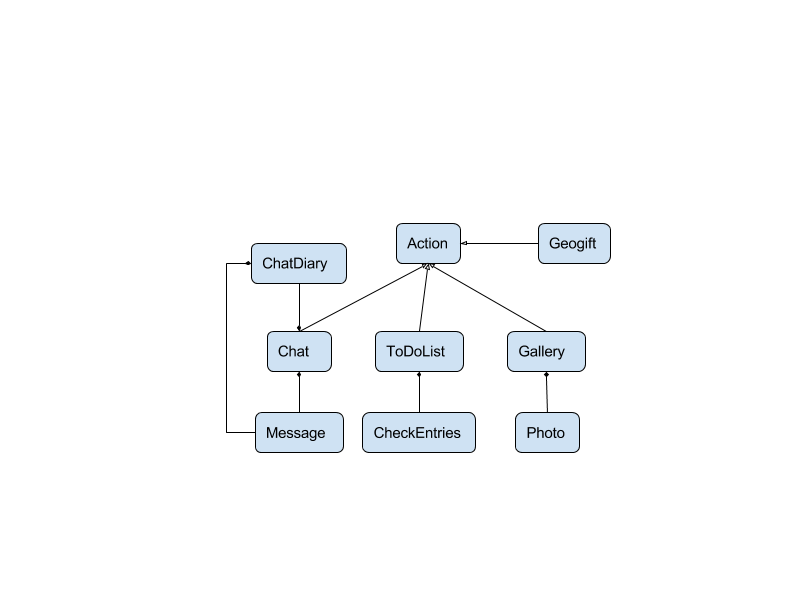
\includegraphics[width=0.50\textwidth, trim={6cm, 6cm, 6cm, 6cm}]{domain}
\end{figure}


\section{App architecture}
\label{sec:app-architecture}

Sweetie could be a long terms project with new extensions in the future so we concentrate a lot of effort to take and maintain a certain architecture in order to keep maintainability and extendability of the app.

Today in the Android community Model View Presenter architecture pattern is the major suggest architecture pattern although the MVP is not a complete architecture pattern as Uncle Bob said in numerous of his talks [].  By the way we would like to clarify that the official Android designer Dianne Hackborn \cite{Dianne_Hackborn_android_arch} doesn't give a precise architecture, Android components by design could be use in very different architecture styles.

In fact the MVP in Android is an element of the Clean Architecture explained very well by his inventor Uncle Bob []. You could see this from the many examples grouped by android community in Android MVP blueprint repository []. We study this example and starts with a simple triad defining by a contract (an interface) of components that are:
View Presenter and Controller
An important aspect is that the View is identified by a Fragment class, next the reference to View meaning the architecture View that is a Fragment, while the presenter is a middle class that keeps independent the Fragment from the model layer of our application. In the Controller we keep all the logic of data and database query, in many architecture the name Controller are substituted with Repository or Service. We don't use Service for not have confusing about the Service component of Android and we don't use Repository word because it means that encapsulated some database logic, in our app the database logic is all into Firebase API so ``repository'' was not valued as a good name choice. 

The activity act like a management of the triad of components of our architecture.
Its responsibility is of instantiate the triad and managed the life cycle of it, in particular when the life cycle go into Destroy or Stop status it must detach the listeners from firebase database in order to avoid memory leak. Because the role of activities is similar, in order to reduce duplicate codes, almost all activity extend a BaseActivity that implements checks and other common functions. Only the LoginActivity doe not extend BaseActivity.

In order to achieve the separation of concern we created for every model data class needed to the View a copy class defined as ViewModel class. The Presenter is the responsible of this conversation that was done when new data come from the Controller. 

For every feature showed in the introduction with the exception of Geogift the application have a triad of classes plus the activity over other utility classes like Adapter and ViewHolder. 

The communication between components of our architecture are always direct calls to method from upper layer (the widget views) and callbacks from lower layer (Controller or android Service) to upper layer except between Views and Presenter.

The communication between Views and Presenter are done through interfaces as the figure~\ref{fig:MVP_image} show. PresenterImp extends Presenter interface that are the reference with which ViewImp communicate, ViewImp extends View interface that are the reference with which PresenterImp communicate.

\begin{figure}[h]
	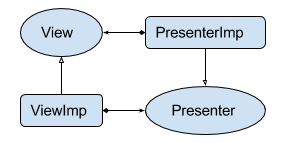
\includegraphics[width=0.5\textwidth, trim={7cm, 7cm, 11cm, 7cm}]{mvp}
	\caption{MVP interface}
	\label{fig:MVP_image}
\end{figure}

The main packages identified a feature of the application and they contain the triad and other utility classes of the feature, for example a DialogFragment.

Aside all pregius of an architecture like MVP we met some difficulties that require the implementations of workaround or a complex solution for a simple task. 

Our need to isolated firebase from other parts of app forced us to use firebase with some limitation. For example Google I/O 2017 available in a open repository in Github [] app use a more complex MVP architecture but the components dependent a lot on firebase API.

Other disadvantages caused by architecture choices are the several callback communication between component, a simple click in a ViewHolder must pass into an Adapter then a Fragment then a Presenter and finally the Controller. By the way we believe that this strong division of relationship between components is a good investments for the future extension of the app.

In the background the app runs four android Service that act like listener to the status of some data into database. 
The UserMonitorService listen when the status of user change, in particular it monitors the relationship status. 
The GeogiftMonitorService manages the life cycle of Geogifts, it downloads them, registers them into LocationService (a Google API Service for monitor location []) and monitors the status of them, if one is destroyed it unregisters it from the LocationServices. When LocationService triggers a Geogift the GeogiftTransitionService acts, it is an IntentService and it create a notification to the user when he discover a Geogift. 
The last Service is the MessagesMonitorService, it monitors the status of all chats and create notifications when new messages are received, it implements a caching system for the notification. The ChatActivity is binded to it in order to reset this notification counter when user enter into a chat.



\section{External API} 

\subsection{Glide}
Glide is a fast and efficient open source media management and image loading framework for Android, we use it for download images and display to the user.

\subsection{Firebase}
Firebase is a powerful platforms that give us a free server with noSQL database and storage and other tools [] and a front-end API which we use it in order to have asynchronous network connection for CRUD operation of our data;

\subsection{MaterialCalendar}
A CalendarView Material look likes, we think that focus on the creation of a Calendar from scratch take too much time.

\subsection{ImagePicker}
Is a library to select single or multiple images from the gallery and camera, used in our Galleries 

\subsection{Image Cropper}
Used for obtain specifical ratio of an image, to set user’s avatar, couple cover,chat and gallery cover.

\subsection{Google Mobile Services API}
Google Mobile Services are a set of library for In particular we use the \texttt{auth} package for Google authentication in app, \texttt{location} and \texttt{places} packages are used for its services of localization and implements our geogift feature and the \texttt{maps} package for the Map section from the main screen of Sweetie.


\section{Main issues}

\subsection{ViewPager with fragment}
The implementation of a ViewPager with a FragmentPagerAdapter for the tab layout in the dashboard of app lead to many problems for managing the lifecycle of the three fragment Diary, Home and Map with the main lifecycle of Dashboard activity.
In some cases we were obligated to use workaround with dirty flag [] and break the division set by the architecture.

\subsection{RecyclerView}
Managed the hierarchies of ViewHolder was a pain, the RecyclerView impose to developer to avoid polymorphism in the creation of ViewHolder and encourage the use of a switch statement with a check on the type represented by an int value, see onCreateViewHolder on android doc []. Fortunately this limitation is only in the creation phase of a ViewHolder, in the binding phase we use the power of polymorphism. Despite of this fact, the RecyclerView, unlike the ListView, give us a more simple flow and an easy managing of the items into the list.

\subsection{Images}
Use image in an Android app and at the same time maintain the usability of it is an very hard task. The Glide library helps us a lot in the download but not in the upload. Firebase API for the upload of files are minimal. The main problems here are:
\begin{itemize}
	\item Upload image and maintain the status progress after Activity is destroyed: we resolve it by change the status of the object into remote server so it persist over the life of the activity, so the both partners see the upload progress;
	\item Reduce the images download time: we don’t implement a compression library into the application but it is necessary for have good usability like WhatsApp, at this moment the first opening of an image it is damn slow.
\end{itemize}

\subsection{Chat keyboard}
As Hackborn said [] the Android SDK doesn’t expected that a developer needs to know when soft keyboard is open, unfortunately this is not the case. In order to create a custom emoticons keyboard interchangeable with soft keyboard we need this information. So we built a workaround and implement a listener that it is triggered when the GlobalLayout object change height, from that we calculate the height of the soft keyboard. In the layout we put a FrameLayout placeholder that use this calculated height for push up the chat items and give space to the custom emoticons keyboard and soft keyboard, in this way the switch between keyboards is pleasant.

% add the bug of first opening



\section{Future Works}

Despite of the great amount of operation that user could do with Sweetie, there are others that we were not able to implement in this version, they are:

\begin{itemize}
	\item Support to other language, in this version the app is in english but the library string get the language set in the system;
	\item The social sharing buttons for make Sweetie less close with user contents;
	\item Build a more robustness notification service, in this version when user kills the application also the service is killed. For do that we will need to run the service into another process;
	\item A local cache system and compress system for images, this is a serious lack because decrease a lot of our  app usability, fortunately Glide reduce this lack but it cache the images only if user previously open them the result is a long wait for the user on the first opening of an image. Over it we need also a compression image library in order to increase the usability and to decrease the use of network connection;
	\item Finally we need to mentions security that will become necessary if the app in the future it will be commercialize through the Google Play Store. In this version the app does not use any type of cryptography for the messages and file uploaded into server neither Firebase database do all the checks that a back-end should do.
\end{itemize}

Working on the project new ideas were born, we describe here the most interesting:

\begin{itemize}
	\item Manage the Geogift discovery with a more smarter way in order to reduce the use of battery and the useless use of localization sensors. For example, the monitoring service should be activated only in proximity of geofence. Improve the experience allowing the sending of Geogifts only in the current physical location and not on remote. Same for the discovering, limited by an expiration time and a distinction between walk and car movements;
	
	\item Import the messages from WhatsApp in order to reduce the barrier of usage from new users;
	
	\item A machine learning engine will learn user actions, in particular which items are bookmarked and saved to diary. Thanks to profiling and user-user matching, the learning could be suggest what elements may be of interest, especially to early adopters on their imported messages;
	
	\item The diary feature that, for us, is still immature and future extensions could bring something more useful for Sweetie’s users. In the future we could implement that every features contributes to filling the diary. User can save the most important (emotionally tied) objects present in the home’s actions like individual messages and photos. The result will be a kind of story that grows in time;
	
	\item Handle the breaking of couples is crucial for maintain active users on the app. One idea is to change main theme of app (different palette colors for example) for an emotional detachment from the relationship just lost, and encourage users to use some dedicated features awaiting a new love story.
\end{itemize}





\section{Conclusion}
\label{sec:conclusion} 
Certainly we can say that Sweetie is a great didactic project. We have needed to learn a lot of android SDK content: Fragment, RecyclerView, ConstraintLayout, Bitmap, ToolBar are only some of classes that we need to learn to manage and use correctly. We also learn to use some powerful Google library that are essential for developing in Android.

We learn also some of the best practices in architecture design for Android. Model View Presenter is a great pattern although we didn't use all the advantages: the testing advantage in particular.

Nevertheless the issues leave open we are satisfied of this release and we are confident that this is the first step for a complete application that can reach the Play Store. Anyway this is only the beginning we should have to learn new components and library of Android for extending our knowledge.


% An example of a floating figure using the graphicx package.
% Note that \label must occur AFTER (or within) \caption.
% For figures, \caption should occur after the \includegraphics.
% Note that IEEEtran v1.7 and later has special internal code that
% is designed to preserve the operation of \label within \caption
% even when the captionsoff option is in effect. However, because
% of issues like this, it may be the safest practice to put all your
% \label just after \caption rather than within \caption{}.
%
% Reminder: the "draftcls" or "draftclsnofoot", not "draft", class
% option should be used if it is desired that the figures are to be
% displayed while in draft mode.
%
%\begin{figure}[!t]
%\centering
%\includegraphics[width=2.5in]{myfigure}
% where an .eps filename suffix will be assumed under latex, 
% and a .pdf suffix will be assumed for pdflatex; or what has been declared
% via \DeclareGraphicsExtensions.
%\caption{Simulation results for the network.}
%\label{fig_sim}
%\end{figure}

% Note that the IEEE typically puts floats only at the top, even when this
% results in a large percentage of a column being occupied by floats.


% An example of a double column floating figure using two subfigures.
% (The subfig.sty package must be loaded for this to work.)
% The subfigure \label commands are set within each subfloat command,
% and the \label for the overall figure must come after \caption.
% \hfil is used as a separator to get equal spacing.
% Watch out that the combined width of all the subfigures on a 
% line do not exceed the text width or a line break will occur.
%
%\begin{figure*}[!t]
%\centering
%\subfloat[Case I]{\includegraphics[width=2.5in]{box}%
%\label{fig_first_case}}
%\hfil
%\subfloat[Case II]{\includegraphics[width=2.5in]{box}%
%\label{fig_second_case}}
%\caption{Simulation results for the network.}
%\label{fig_sim}
%\end{figure*}
%
% Note that often IEEE papers with subfigures do not employ subfigure
% captions (using the optional argument to \subfloat[]), but instead will
% reference/describe all of them (a), (b), etc., within the main caption.
% Be aware that for subfig.sty to generate the (a), (b), etc., subfigure
% labels, the optional argument to \subfloat must be present. If a
% subcaption is not desired, just leave its contents blank,
% e.g., \subfloat[].


% An example of a floating table. Note that, for IEEE style tables, the
% \caption command should come BEFORE the table and, given that table
% captions serve much like titles, are usually capitalized except for words
% such as a, an, and, as, at, but, by, for, in, nor, of, on, or, the, to
% and up, which are usually not capitalized unless they are the first or
% last word of the caption. Table text will default to \footnotesize as
% the IEEE normally uses this smaller font for tables.
% The \label must come after \caption as always.
%
%\begin{table}[!t]
%% increase table row spacing, adjust to taste
%\renewcommand{\arraystretch}{1.3}
% if using array.sty, it might be a good idea to tweak the value of
% \extrarowheight as needed to properly center the text within the cells
%\caption{An Example of a Table}
%\label{table_example}
%\centering
%% Some packages, such as MDW tools, offer better commands for making tables
%% than the plain LaTeX2e tabular which is used here.
%\begin{tabular}{|c||c|}
%\hline
%One & Two\\
%\hline
%Three & Four\\
%\hline
%\end{tabular}
%\end{table}


% Note that the IEEE does not put floats in the very first column
% - or typically anywhere on the first page for that matter. Also,
% in-text middle ("here") positioning is typically not used, but it
% is allowed and encouraged for Computer Society conferences (but
% not Computer Society journals). Most IEEE journals/conferences use
% top floats exclusively. 
% Note that, LaTeX2e, unlike IEEE journals/conferences, places
% footnotes above bottom floats. This can be corrected via the
% \fnbelowfloat command of the stfloats package.





% if have a single appendix:
%\appendix[Proof of the Zonklar Equations]
% or
%\appendix  % for no appendix heading
% do not use \section anymore after \appendix, only \section*
% is possibly needed

% use appendices with more than one appendix
% then use \section to start each appendix
% you must declare a \section before using any
% \subsection or using \label (\appendices by itself
% starts a section numbered zero.)
%


%\appendices
%\section{Proof of the First Zonklar Equation}
%Appendix one text goes here.

% you can choose not to have a title for an appendix
% if you want by leaving the argument blank
%\section{}
%Appendix two text goes here.


% use section* for acknowledgment
%\section*{Acknowledgment}


%The authors would like to thank...


% Can use something like this to put references on a page
% by themselves when using endfloat and the captionsoff option.
\ifCLASSOPTIONcaptionsoff
  \newpage
\fi



% trigger a \newpage just before the given reference
% number - used to balance the columns on the last page
% adjust value as needed - may need to be readjusted if
% the document is modified later
%\IEEEtriggeratref{8}
% The "triggered" command can be changed if desired:
%\IEEEtriggercmd{\enlargethispage{-5in}}

% references section


% can use a bibliography generated by BibTeX as a .bbl file
% BibTeX documentation can be easily obtained at:
% http://mirror.ctan.org/biblio/bibtex/contrib/doc/
% The IEEEtran BibTeX style support page is at:
% http://www.michaelshell.org/tex/ieeetran/bibtex/
%\bibliographystyle{IEEEtran}
% argument is your BibTeX string definitions and bibliography database(s)
%\bibliography{bib/paper}
%
% <OR> manually copy in the resultant .bbl file
% set second argument of \begin to the number of references
% (used to reserve space for the reference number labels box)
\begin{thebibliography}{1}
	
	\bibitem{IEEEhowto:kopka}
	H.~Kopka and P.~W. Daly, \emph{A Guide to \LaTeX}, 3rd~ed.\hskip 1em plus
	0.5em minus 0.4em\relax Harlow, England: Addison-Wesley, 1999.
	
	\bibitem{Android MVP blueprints}
	Android MVP blueprints repository \url{https://github.com/googlesamples/android-architecture}
	
	\bibitem{citekey}
	
	
\end{thebibliography}




% that's all folks
\end{document}


